% 旋转体的体积, solid of revolution
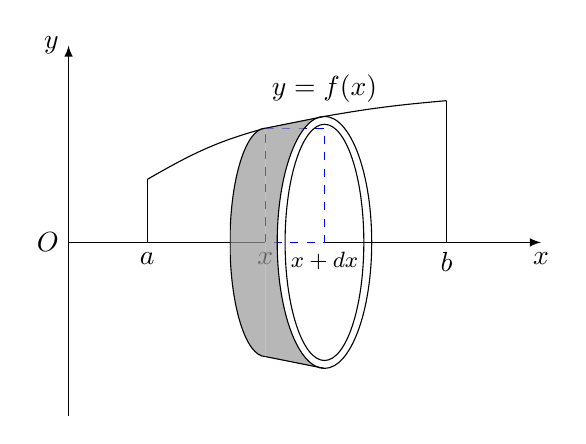
\begin{tikzpicture}[scale=1]
  % \draw [help lines] (-3,-3) grid (3,3);

  % 坐标
  \node[left] at (0,2.5) {$y$};
  \draw[-latex] (0,-2.2) -- (0,2.5);
  \node[below] at (6,0) {$x$};
  \draw (0,0) -- (2.5,0);
  \draw[-latex] (3.25,0) -- (6,0);
  \node[left] at (0,0) {$O$};

  % y=f(x)
  \node[above] at (3.25,1.65) {$y=f(x)$};
  \draw (1,0.8) to [out=30,in=195] (2.5,1.45);
  \draw (3.25,1.6) to [out=10,in=185] (4.8,1.8);

  % 端点
  \node[below] at (1,0) {$a$};
  \draw (1,0.8) -- (1,0);
  \node[below] at (4.8,0) {$b$};
  \draw (4.8,1.8) -- (4.8,0);

  \node[below] at (2.5,0) {$x$};
  \node[below] at (3.25,0) {\footnotesize $x + dx$};
  \draw[dashed, blue] (2.5,1.45) -- (3.25,1.45) -- (3.25,0) -- (2.5,0) -- (2.5,1.45);

  % ----------------------------------------------------------------------------

  % 左边椭圆和填充
  \begin{scope}
    \pgfsetfillopacity{0.7}
    \clip (2.05,-1.47) rectangle (2.501,1.47);
    \draw[fill=black!40] (2.5,0) ellipse [x radius=0.45cm,y radius=1.45cm];
  \end{scope}
  % 填充
  \begin{scope}
    \clip (2.4,-1.6) rectangle (3.24,1.6); % 3.25 --> 3.24,移除精度导致的黑线
    \pgfsetfillopacity{0.7}
    \path[fill=black!40,even odd rule] (2.5,1.45) -- (3.25,1.6) -- (3.25,-1.6) -- (2.5,-1.45) -- (2.5,1.45)
    (3.25,0) ellipse [x radius=0.6cm,y radius=1.6cm];
  \end{scope}

  % 右边椭圆
  \draw (3.25,0) ellipse [x radius=0.6cm,y radius=1.6cm];
  \draw (3.25,0) ellipse [x radius=0.5cm,y radius=1.5cm];

  % 椭圆上下边线
  \draw (2.5,1.45) -- (3.25,1.6);
  \draw (2.5,-1.45) -- (3.25,-1.6);
\end{tikzpicture}
